\chapter{Introducción}

En este trabajo se obtuvo un diseño preliminar para sistemas de intercambio de
gases del \gls{mrcvc} \cite{toth}, optimizando el rendimiento volumétrico con
una curva de rendimiento requerido seleccionada provisoriamente.
%
Se realizó una primer aproximación utilizando coeficientes de descarga (Cd)
estimados en trabajos anteriores \cite{lopez13} para simular el ciclo
termodinámico del motor con el simulador de motores de combustión interna ICESym
\cite{icesym}.
%
Con el valor estimados de Cd para ambos puertos se optimizó diámetros,
longitudes y reglaje de los puertos, la optimización se realizó utilizando un
algoritmo genético que modela motores como individuos y da puntaje a cada uno
comparando las curvas de rendimiento volumétrico con la curva requerida ,
cuanto más parecida la curva de cada motor con la curva objetivo, mayor
puntaje.


El diseño preliminar se volcó en un diseño 3D de los puertos de admisión y
escape, con estos modelos se realizó una serie de flujometrías con el objetivo
de obtener un mapa del coeficiente de descarga en función de dos variables:
alzada equivalente y diferencia de presión.
%
El mapa de Cd se utilizó como retroalimentación del simulador ICESym para
repetir los pasos descritos anteriormente y luego de algunas iteraciones se
obtuvo un diseño satisfactorio.

La motivación de este trabajo surge de continuar con el desarrollo del MRCVC,
en particular mejorar el prediseño de los sistemas de intercambio de gases
sentando las bases para una futura optimización de los mismos en un motor con
requisitos de diseño establecidos.
%
El MRCVC es un proyecto nacido en la Universidad Nacional del Comahue en el
marco del \emph{Proyecto de Investigación Desarrollo de modelos y herramientas
para la simulación de problemas complejos en ingeniería mediante fluido dinámica
computacional (04/I-251)}. Actualmente se encuentra en etapa de desarrollo.

\begin{figure}[h!]
    \centering
    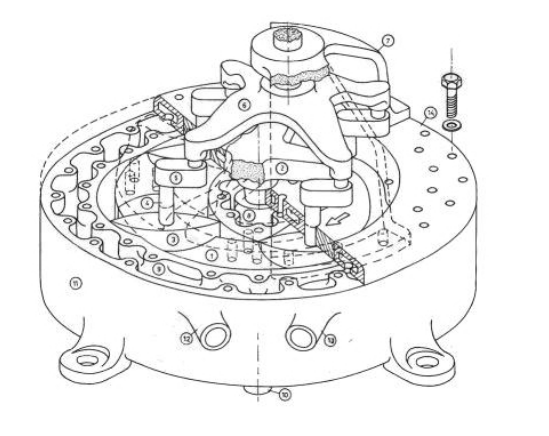
\includegraphics[width=0.5\textwidth]{perspectiva_mrcvc.png}
    \caption{Motor Rotativo de Combustión a Volumen Constante}
    \label{fig:mrcvc}
\end{figure}
